\documentclass{article}

\usepackage{graphicx}
\usepackage{indentfirst}
\usepackage[a4paper, total={6in, 8in}]{geometry}
\usepackage{hyperref}
\usepackage{fancyhdr}
\usepackage{xepersian}
\usepackage{fontspec}
\usepackage{url}
\settextfont{B Nazanin}
\setlatintextfont{Times New Roman}

\begin{document}


%title page%
\begin{titlepage}
	\begin{center}
		\vspace{0.2cm}
		
		
\includegraphics[width=0.4\textwidth]{sharif.png}\\
		\vspace{0.5cm}
		\textbf{ \Huge{فاز اول}}\\
		\vspace{0.25cm}
		\textbf{ \Large{پروژه مقدمه‌ای بر بیوانفورماتیک - دکتر علی  شریفی‌زارچی و دکتر سمیه کوهی}}
		\vspace{0.2cm}
		
		
		\large \textbf{دانشکده مهندسی کامپیوتر}\\\vspace{0.1cm}
		\large   دانشگاه صنعتی شریف\\\vspace{0.2cm}
		\large   ﻧﯿﻢ‌سال اول ۰۱-۰۲ \\\vspace{0.2cm}
		\large{\Large{امیرحسین باقری - 98105621}}\\
		\large{\Large{مهدی مستانی - 97100513}}\\
		\large{\Large{محمدرضا مفیضی - 98106059}}\\
	\end{center}
\end{titlepage}
%title page%

\newpage

%pages header
\pagestyle{fancy}
\fancyhf{}
\fancyfoot{}
\setlength{\headheight}{59pt}
\cfoot{\thepage}
\lhead{فاز اول}
\rhead{
\includegraphics[width=0.1\textwidth]{sharif.png}\\
		دانشکده مهندسی کامپیوتر
}
\chead{پروژه مقدمه‌ای بر بیوانفورماتیک}
%pages header

\section{ریزآرایه چیست؟}
ریزآرایه \LTRfootnote{\lr{microarray}}، ابزاری آزمایشگاهی است که برای تشخیص بیان هزاران ژن به طور همزمان استفاده می‌شود. ریزآرایه‌های \lr{DNA} لام‌های میکروسکوپی هستند که با هزاران نقطه کوچک در موقعیت‌های مشخص چاپ می‌شوند و هر نقطه حاوی یک توالی \lr{DNA} یا ژن شناخته‌شده است.

 \subsection*{روش کار}
برای انجام تحلیل ریزآرایه، مولکول‌های \lr{mRNA} معمولاً از هر دو نمونه آزمایشی و نمونه مرجع جمع‌آوری می‌شوند. به عنوان مثال، نمونه مرجع را می‌توان از یک فرد سالم، و نمونه آزمایشی را می‌توان از یک فرد مبتلا به بیماری مانند سرطان جمع‌آوری کرد. سپس دو نمونه \lr{mRNA} به \lr{DNA} مکمل (\lr{cDNA}) تبدیل می‌شوند و هر نمونه با یک ترکیب فلورسنت \LTRfootnote{\lr{fluorescent}} با رنگ متفاوت برچسب‌گذاری می‌شود. مثلا، نمونه آزمایشی \lr{cDNA} ممکن است با رنگ فلورسنت قرمز برچسب‌گذاری شود، در حالی که \lr{cDNA} مرجع با رنگ فلورسنت سبز برچسب‌گذاری می‌شود.

 سپس دو نمونه با هم مخلوط شده و اجازه داده می‌شود تا به لام ریزآرایه متصل شوند. فرآیندی که در آن مولکول‌های \lr{cDNA} به ترکیب‌های \lr{DNA} روی لام متصل می‌شوند، هیبریداسیون \LTRfootnote{\lr{hybridization}} نامیده می‌شود.
پس از هیبریداسیون، ریزآرایه برای اندازه‌گیری میزان بیان هر ژن چاپ‌شده روی لام اسکن می‌شود. اگر بیان یک ژن خاص در نمونه آزمایشی بیشتر از نمونه مرجع باشد، نقطه مربوطه روی ریزآرایه قرمز به نظر می‌رسد.
از طرفی، اگر بیان در نمونه آزمایشی کمتر از نمونه مرجع باشد، آن نقطه سبز به نظر می‌رسد. در نهایت، اگر میزان بیان در دو نمونه یکسان باشد، نقطه زرد خواهد بود. داده‌های جمع‌آوری‌شده از طریق ریزآرایه‌ها را می‌توان برای ایجاد پروفایل‌های بیان ژن، که تغییرات همزمان در بیان بسیاری از ژن‌ها در پاسخ به یک بیماری یا درمان خاص را نشان می‌دهد، استفاده کرد. \cite{nature-microarray}
 
 \subsection*{فرمت داده‌‌های خروجی}
مجموعه داده‌های ریزآرایه معمولاً بسیار بزرگ هستند و فرمت داده‌های خروجی به صورت یک فایل خام (\lr{Raw Matrix}) در قالب یک متن \lr{tab-seperated} حاوی داده‌های بیش از یک سنجش ترکیبی (ترکیب‌ها در سطر‌ و نتایج آزمایش‌ها در ستون) است.
در تصویر \ref{fig:microarray} میزان بیان هر ژن به صورت \lr{heatmap} نمایش داده شده است.
\begin{figure}[h!]
	\centering
	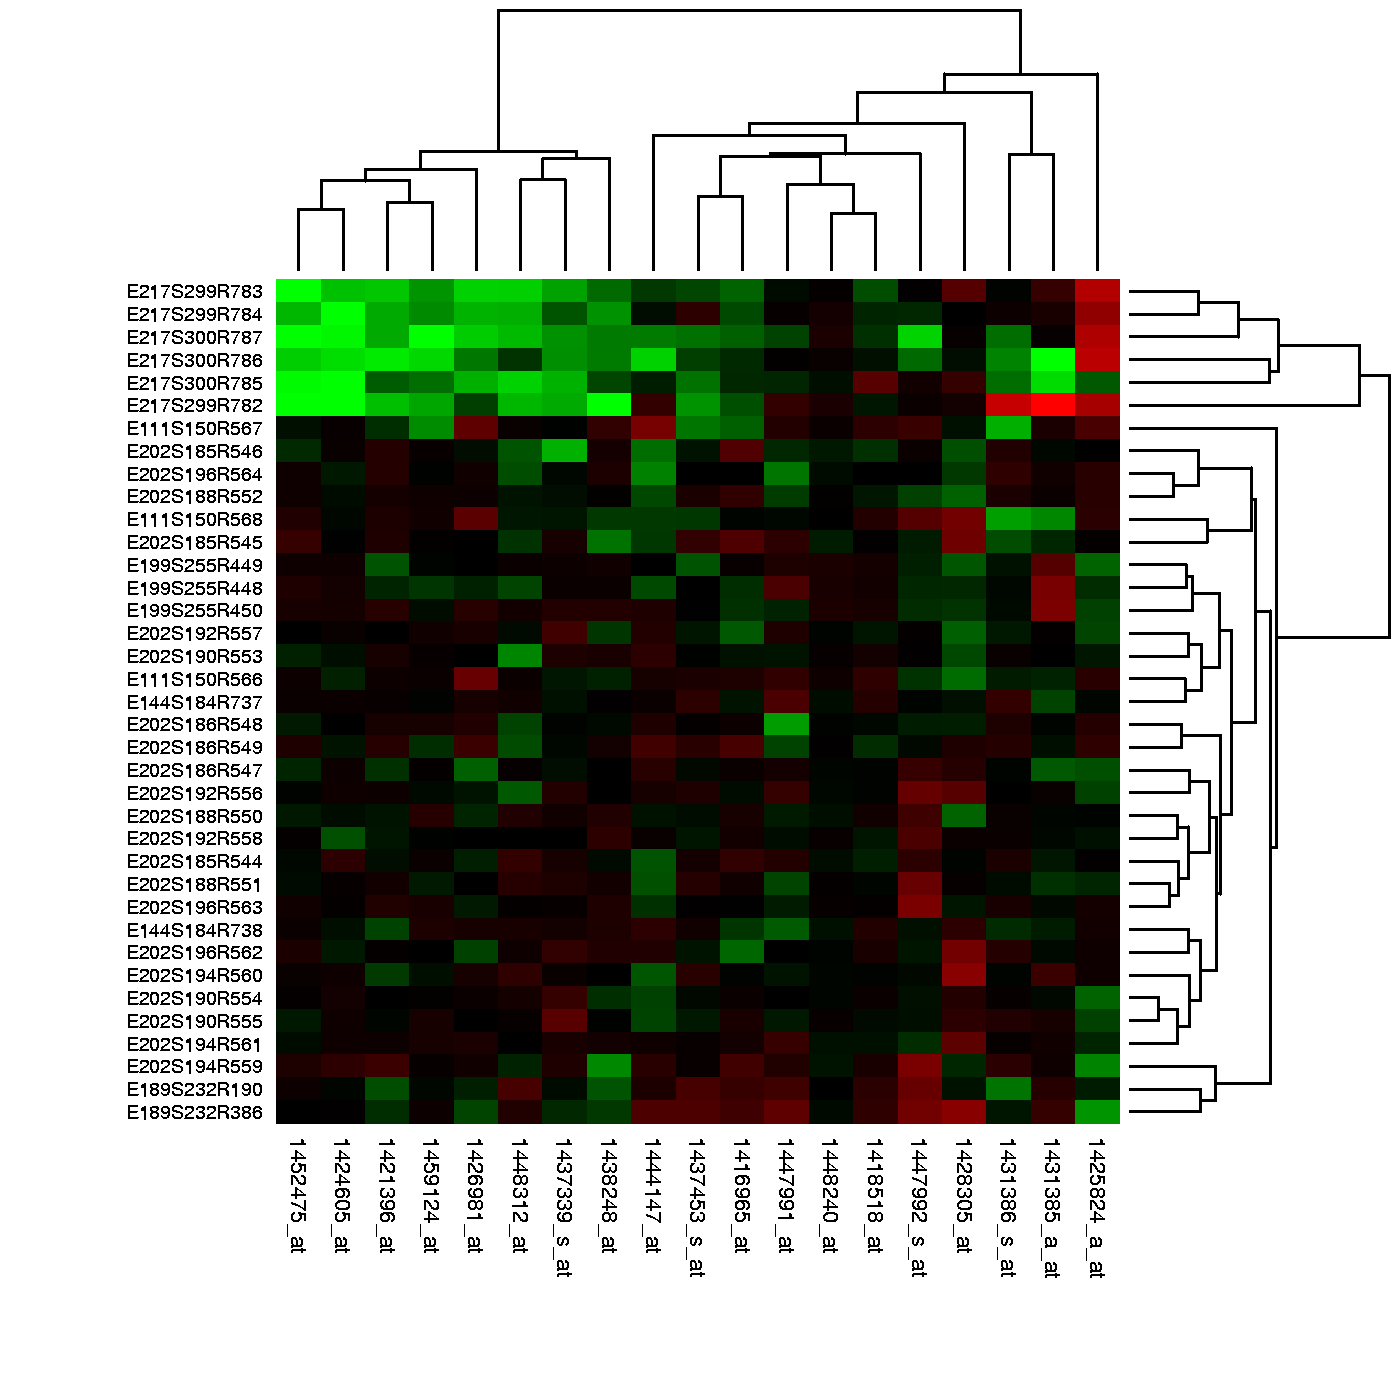
\includegraphics[width=0.3\columnwidth]{figs/microarray.png}
	\caption{میزان بیان ژن در ریزآرایه \cite{wiki-microarray}}
	\label{fig:microarray}
\end{figure}

\section{کیفیت داده‌ها}
پس

\section{کاهش ابعاد داده‌‌ها}
پس
\section{همبستگی بین گروه‌ها}
پس

\newpage
\begin{thebibliography}{99}
	\begin{latin}
		\bibitem{nature-microarray}
		Nature Defenition Microarray (2014), Nature Education, \url{https://www.nature.com/scitable/definition/microarray-202}
		
		\bibitem{wiki-microarray}
		Microarray Hitmap (2006), Wikipedia, \url{https://commons.wikimedia.org/wiki/File:Heatmap.png#/media/File:Heatmap.png}
		
%		\bibitem{lamport94}
%		Leslie Lamport (1994) \emph{\LaTeX: a document preparation system}, Addison
%		Wesley, Massachusetts, 2nd ed.
	\end{latin}
\end{thebibliography}



\end{document}
